\section{Energy integration}


Nasibeh use cetow for heat puming solutions and st fons for large scale integration and combined heat and power production. We have to use neutralised values (i.e. we start with 100 unit and end up with 46.


Converting energy resources into useful energy, exergy efficiency, heat pumping and combined heat and power => examples from the papers of Nasibeh

adding a citation \cite{Pouransari_2014_1}

testing equations
\begin{equation}
min \, obj= \frac{things_{good}}{things_{bad}} \forall things\\
\text{subject to}  \\
things_{bad}\ge necessary\,\, level \cup unnecessary \, level
\end{equation}

**************

\subsection{Caste study I: Energy integration technologies}

The process heat transfer requirement for a real chemical site is defined for each process unit operation using multi-level data extraction approach of \cite{Pouransari_2014_2}. 

        \begin{figure}[h]
        \begin{center}
        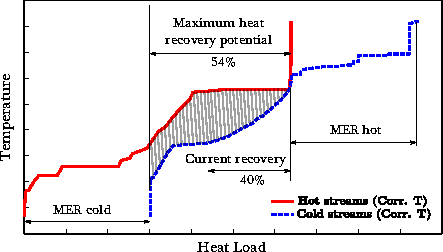
\includegraphics [height=4.3cm]{figures/EnergyIntegration/figMERcc.pdf} 
        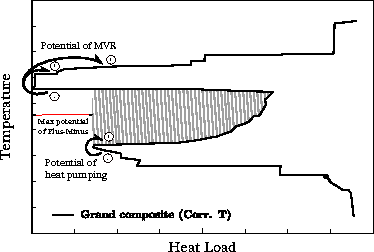
\includegraphics [height=4.3cm]{figures/EnergyIntegration/figMERgcc.pdf}
        \caption{Composite and Grand Composite Curves of the process after heat integration}
        \label{fig1:mer}
        \end{center}
        \end{figure}
        


      \begin{figure}[h]
      \begin{center}
      \begin{tabular}{cc}
        \subfloat[With MVR]{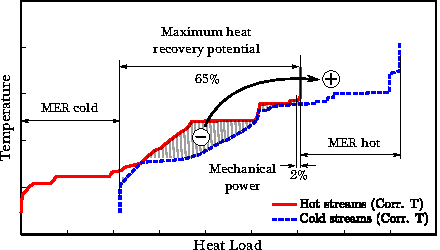
\includegraphics [height=4cm]{figures/EnergyIntegration/HPmvr_mvralone.pdf}} & 
        \subfloat[With MVR and HP]{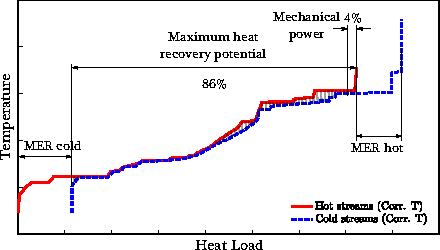
\includegraphics [height=4cm]{figures/EnergyIntegration/HPmvr_mvrhp.pdf}}
       \end{tabular}
      \caption{Composite Curves after improvement potentials}
      \label{fig1:HPmvr}
      \end{center}
      \end{figure}
